\documentclass{nordic}
\usepackage[utf8]{inputenc}
\usepackage{graphicx}
\usepackage{amsmath}
\usepackage[colorlinks=true,linkcolor=black,citecolor=black,urlcolor=black]{hyperref}

% Changes applied / Mikael Öhman, Chalmers University of technology, mikael.ohman@chalmers.se
% * Corrected summary spacing according to document, no more vskips in side the latex document.
% * Corrected float spacing according to text. No need for any vskip, always correct. This wasn't even correct in the old document.
% * Natbib for citing instead of manual superscripts (biblatex is probably still to new, but could be used).
% * Using textsuperscript instead of abusing math mode.
% * Real urls. If you want urls in the address field, \AtBeginDocument can't place \maketitle.
% * Bibtex file instead of writing them manually. 
% * Removed all eps-hacks. pdflatex should be used in favour of latex.
% * New commands to help update the document easily (seeing how the old document was outdated in some places).

% If you are new to LaTeX, see up-to-date usage of LaTeX at: http://en.wikibooks.org/wiki/LaTeX
% Also be sure to read the amsmath manual, TikZ/PGF/pgfplots for figures, tabularx for advanced tables. 

\newcommand{\NSCM}{23}
\newcommand{\submissionyear}{2010}
\newcommand{\submissiondate}{September 15th 2010}
\newcommand{\submissionpage}{http://congress.cimne.upc.es/nscm-\NSCM/frontal}

\header{
  \NSCM rd Nordic Seminar on Computational Mechanics\\
  NSCM-\NSCM\\
  A. Eriksson and G. Tibert (Eds)\\
  \copyright KTH, Stockholm, \submissionyear
}

\title{INSTRUCTIONS TO PREPARE AN EXTENDED ABSTRACT FOR THE
 \NSCM\textsuperscript{rd} NORDIC SEMINAR ON COMPUTATIONAL MECHANICS\break NSCM-\NSCM}

\author{First A. Author$^*$, Second B. Author$^\dag$ and Third C. Coauthor$^\dag$}

\heading{First A. Author, Second B. Author and Third C. Coauthor}

\address{$^*$International Center for Numerical Methods in Engineering (CIMNE)\\
Universidad Polit\'ecnica de Catalu\~na\\
Campus Norte UPC, 08034 Barcelona, Spain\\
e-mail: \url{congreso@cimne.upc.edu}, web page: \url{http://www.cimne.upc.com/}
\and
$^\dag$Spanish Association for Numerical Methods in Engineering (SEMNI)\\
Edificio C1, Campus Norte UPC\\
Gran Capit\'an s/n, 08034 Barcelona, Spain\\
e-mail: \url{semni@cimne.upc.edu} - Web page: \url{http://www.semni.org}}

\keywords{Marine Engineering, Computational Techniques, Applications, Computational Methods.}

\abstract{%
This document provides information and instructions for
preparing an Extended Abstract to be included in the Proceedings
of \textit{NSCM-\NSCM}. It can be written in Word.
}

\begin{document}
\maketitle

\section{INTRODUCTION}

The Seminar publication will consist of a hard-printed book
containing Extended Abstracts of the contributions received.
Authors should submit the Extended Abstract electronically via the
web page of the Conference,
\underline{\url{\submissionpage}} before \submissiondate.
The Extended Abstract should be written following the
format of Word macros for submission that can be found in that
address. The file has to be translated into Portable Document
Format (PDF) before submission via the Conference site. The
organizers do not commit themselves to include in the Proceedings
any Extended Abstract received later than the above-mentioned
deadline. The speaker and the contact author should match. The
speaker must register and pay his registration fee during the
advance period (before \submissiondate) for the Extended
Abstract to be included in the final programme of the Seminar.

\section{GENERAL ESPECIFICATIONS}

The Extended Abstract must be written in English within a printing
box of 16cm x 21cm, centered in the page. The Extended Abstract
including figures, tables and references must have a minimum
length of 2 pages and must not exceed 4 pages. Maximum file size
is 4 MB.

\section{TITLE, AUTHORS, AFFILIATION, KEY WORDS}

The first page must contain the Title, Author(s), Affiliation(s),
Key words and the Summary. The Introduction must begin immediately
below, following the format of this template.

\subsection{Title}

The title should be written centered, in 14pt, boldface Roman, all
capital letters. It should be single spaced if the title is more
than one line long.

\subsection{Author}

The author's name should include first name, middle initial and
surname. It should be written centered, in 12pt boldface Roman,
12pt below the title.

\subsection{Affiliation}

Author's affiliation should be written centered, in 11pt Roman,
12pt below the list of authors. A 12pt space should separate two
different affiliations.

\subsection{Key words}

Please, write no more than six key words. They should be written
left aligned, in 12pt Roman, and the line must begin with the
words Key words: boldfaced. A 12pt space should separate the key
words from the affiliations.

\subsection {Summary (optional)}

Use 12pt Italic Roman for the summary. The word Summary must be
set in boldface, not italicized, at the beginning of the first
line. The text should be justified and separated 12pt from the key
words, as shown in the first page of these instructions.

\section{HEADINGS}

\subsection{Main headings}

The main headings should be written left aligned, in 12pt,
boldface and all capital Roman letters. There should be a 12pt
space before and 6pt after the main headings.

\subsection {Secondary headings}

Secondary headings should be written left aligned, 12pt, boldface
Roman, with an initial capital for first word only. There should
be a 12pt space before and 6pt after the secondary headings.

\section{EDITORIAL HEADING}

The first page has to include the Editorial Heading, as shown in
the first page of these instructions. Successive pages will
include the name of the authors.

\section{TEXT}

The normal text should be written single-spaced, justified, using
12pt (Times New) Roman in one column. The first line of each
paragraph must be indented 0.5cm. There is not inter-paragraph
spacing.

\section{PAGE NUMBERS}

In order to organize the Extended Abstract, it is better to number
the pages. Page numbers are not included in the printing box.

\section{FIGURES}

All figures should be numbered consecutively and captioned. The
caption title should be written centered, in 10pt Roman, with
upper and lower case letters.
\begin{figure}[h!]
\centering
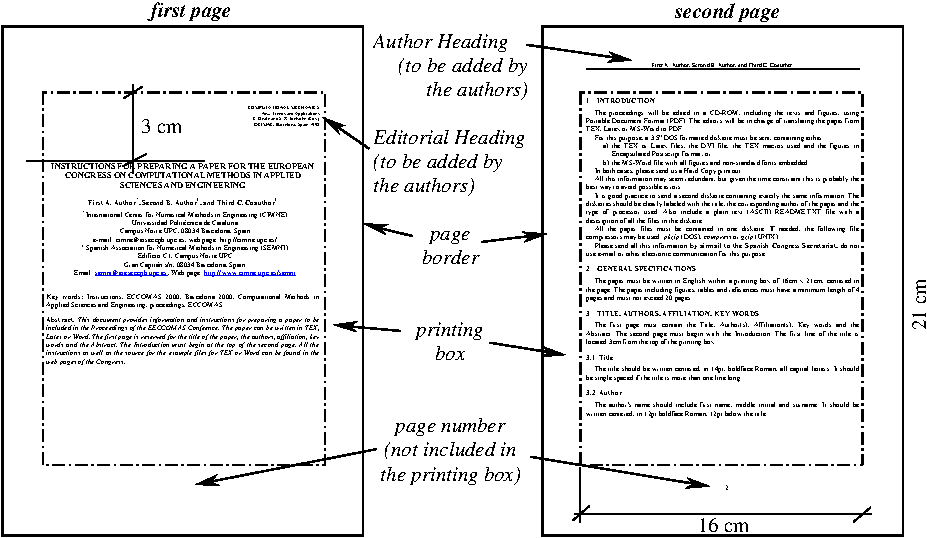
\includegraphics[width=10cm]{firstpage.pdf}
\caption{Page layout}
\end{figure}

A 6pt space should separate the figure from the caption, and a
12pt space should separate the upper part of the figure and the
bottom of the caption from the surrounding text.

Figures may be included in the text or added at the bottom of the
Extended Abstract.


\section{EQUATIONS}

A displayed equation is numbered, using Arabic numbers in
parentheses. It should be centered, leaving a 6pt space above and
below to separate it from the surrounding text.

The following example is a single line equation:

\begin{equation}
Ax = b
\end{equation}
\eject

The next example is a multi-line equation (see the amsmath nmanual for more examples):

\begin{align}
Ax &= b \\
Ax &= b \nonumber
\end{align}

\section{TABLES}

All tables should be numbered consecutively and captioned, the caption should be 10pt Roman, upper and lower
case letters.

\begin{table}[h!]
\centering
\begin{tabular}{*{3}{|c}|} % See tabularx for more advanced typesetting
\hline
C11 & C12 & C13 \\
\hline
C21 & C22 & C23 \\
\hline
C31 & C32 & C33 \\
\hline
C41 & C42 & C43 \\
\hline
C51 & C52 & C53 \\
\hline
\end{tabular}
\caption{Example of the construction of one table}
\end{table}

A 6pt space should separate the table from the caption, and a 12pt space should separate the table from the
surrounding text.

\section{FORMAT OF REFERENCES}

References should be quoted in the text by superscript numbers\cite{Zienkiewicz,Idelsohn}, and  grouped together at the end of
the Extended Abstract in numerical order as shown in these instructions.

\section{CONCLUSIONS}

\begin{enumerate}
\item Extended Abstracts in format for publication should be submitted electronically via the web page of the
Conference \url{\submissionpage} , before \submissiondate.
They must be translated into Portable Document Format (PDF) before submission.
The maximum size of the file is 4 MB.

\item The speaker (contact author) should register and pay his registration fee during the advance period
(before \submissiondate) for their Extended Abstract
to be included in the final programme of the Conference.
\end{enumerate}

\bibliography{references.bib}
\bibliographystyle{naturemag}
% If the style is missing from your tex distribution, get it at;
% http://www.ctan.org/tex-archive/macros/latex/contrib/nature/

% Old manually typed bibliography;
%\begin{thebibliography}{99}
%\bibitem{Zienkiewicz} O.C. Zienkiewicz and R.L. Taylor, \textit{The finite element method}, McGraw Hill,
%Vol. I., (1989), Vol. II., (1991).
%\bibitem{Idelsohn} S. Idelsohn and E. O\~nate. Finite element and finite volumes. Two good friends.
%\textit{Int. J. Num. Meth. Engng.}, \textbf{37}, 3323--3341, (1994).
%\end{thebibliography}

\end{document}

